%************************************************
\chapter{Introduction}\label{ch:introduction}
%************************************************
\glsresetall % Resets all acronyms to not used

\ac{AnSiAn} is an Android application by the Secure Mobile Network Lab (SEEMOO) at 
Technische Universität Darmstadt. It features a graphical signal analyzer that can be used with common \acp{SDR} like the
HackRF and the RTL-SDR. The project is based on RF~Analyzer, an application by
Dennis Mantz. \ac{AnSiAn} currently extends RF~Analyzer by the following features: 
\begin{itemize}
	\item Time Domain Signal Graph (Waveform)
	\item Morse Decoder
	\item Scanner
	\item Codebase structured according to the \ac{MVC} pattern
\end{itemize}

This lab aims to further extend the feature set of \ac{AnSiAn} while also
making the app more stable and refining existing features. The description of
the project goals are listed in \autoref{sec:project_definition}.


\section{Project Definition\label{sec:project_definition}}

This section defines the features that will be implemented throughout the
project and schedules them into three sprints.

\subsection{Features}

The new features can be divided into mandatory features, that will have high
priority within this project, and optional features, that will be implemented
if time permits. As can be seen in \autoref{sec:time_schedule}, the third
sprint is reserved for either optional features or completing mandatory
features and the documentation.

\subsubsection{Mandatory Features}

The following features are scheduled for implementation during the first and
second sprint:
\begin{itemize}
	\item \ac{RDS} demodulation \\
		If the user selects the existing wide-band \ac{FM} demodulation option,
		the app shall try to detect and demodulate any existing \ac{RDS}
		signal along with the audio demodulation. The extracted information
		shall be displayed on the screen.
	\item \ac{PSK31} demodulation \\
		If the user selects either of the single side band demodulation modes
		(\ac{USB} and \ac{LSB}), he or she shall have the option to enable
		\ac{PSK31} demodulation along with or instead of the audio demodulation.
		The demodulated text string shall appear and scroll through the
		analyzer window.
	\item Extraction of RDS-, Morse- and \ac{PSK31}-data to logfiles \\
		If the user selects to demodulate any digital mode, the demodulated
		text shall be written to a log file specified by the user.
	\item Support for the rad1o badge \\
		The rad1o badge, which is a modified low-cost replica of the HackRF,
		shall be supported as a signal source by \ac{AnSiAn}.
	\item Transmission support for HackRF and rad1o \\
		If \ac{AnSiAn} is used with an \ac{SDR} capable of transmitting signals,
		it shall offer options to send signals in the following ways:
		\begin{itemize}
			\item Replay I/O samples from a file
			\item Generate and send Morse code from text
			\item FM-modulate and send audio from a file
		\end{itemize}
\end{itemize}

\subsubsection{Optional Features}

The optional features are scheduled in the third and last sprint. However,
they will only be added to the feature set if the last sprint is not needed
in order to compensate for delays on the mandatory features. The optional features are
listed in the order of priority:
\begin{itemize}
	\item Walkie-Talkie Mode \\
		The user shall have the possibility to put \ac{AnSiAn} into a Walkie-
		Talkie mode. In this mode, the application will demodulate an FM channel
		and the user can quickly switch between demodulation and transmission
		of audio recorded from the internal microphone.
	\item Packet Radio demodulation\\
		A new mode \emph{Packet Radio} shall be added to \ac{AnSiAn}. Once selected, it shall allow the user
		to tune to a Packet Radio channel and display information about 
		demodulated packets on the screen. If time permits, it might even
		be possible to implement a transmission feature for Packet Radio.
\end{itemize}


\subsection{Time Schedule}
\label{sec:time_schedule}

The project will have two developers, Dennis Mantz and Max Engelhardt,
working in three sprints. There are three milestones corresponding to
the sprints, labeled Alpha, Beta and Final Version. They each add an independent
and self-contained set of features to the application:

\begin{itemize}
	\item Software Design (due 12.05.)
	\item Sprint 1: Alpha Version (due 09.06.)
	\begin{itemize}
		\item \ac{RDS} demodulation
		\item \ac{PSK31} demodulation
		\item Extraction of \ac{RDS}-, Morse- and \ac{PSK31}-data to logfiles
	\end{itemize}
	\item Sprint 2: Beta Version (due 21.07.)
	\begin{itemize}
		\item Support for the rad1o badge
		\item Transmission support for HackRF and rad1o
		\begin{itemize}
			\item Replay I/O samples from a file
			\item Generate and send Morse code from text
			\item FM-modulate and send audio from a file
		\end{itemize}
	\end{itemize}
	\item Sprint 3: Final Version (due 25.08.)
	\begin{itemize}
		\item Complete leftovers from previous sprints
		\item Walkie-Talkie Mode (optional)
		\item Packet Radio demodulation (optional)
	\end{itemize}
\end{itemize}

\section{Cleanup Tasks\label{sec:cleanup}}

Outside the scope of the planned sprints, some cleanup tasks were necessary
to prepare the implementation of the features listed in
\autoref{sec:project_definition}.

\subsection{Memory Optimizations\label{sec:cleanup.mem}}

\begin{figure}
	\centering
	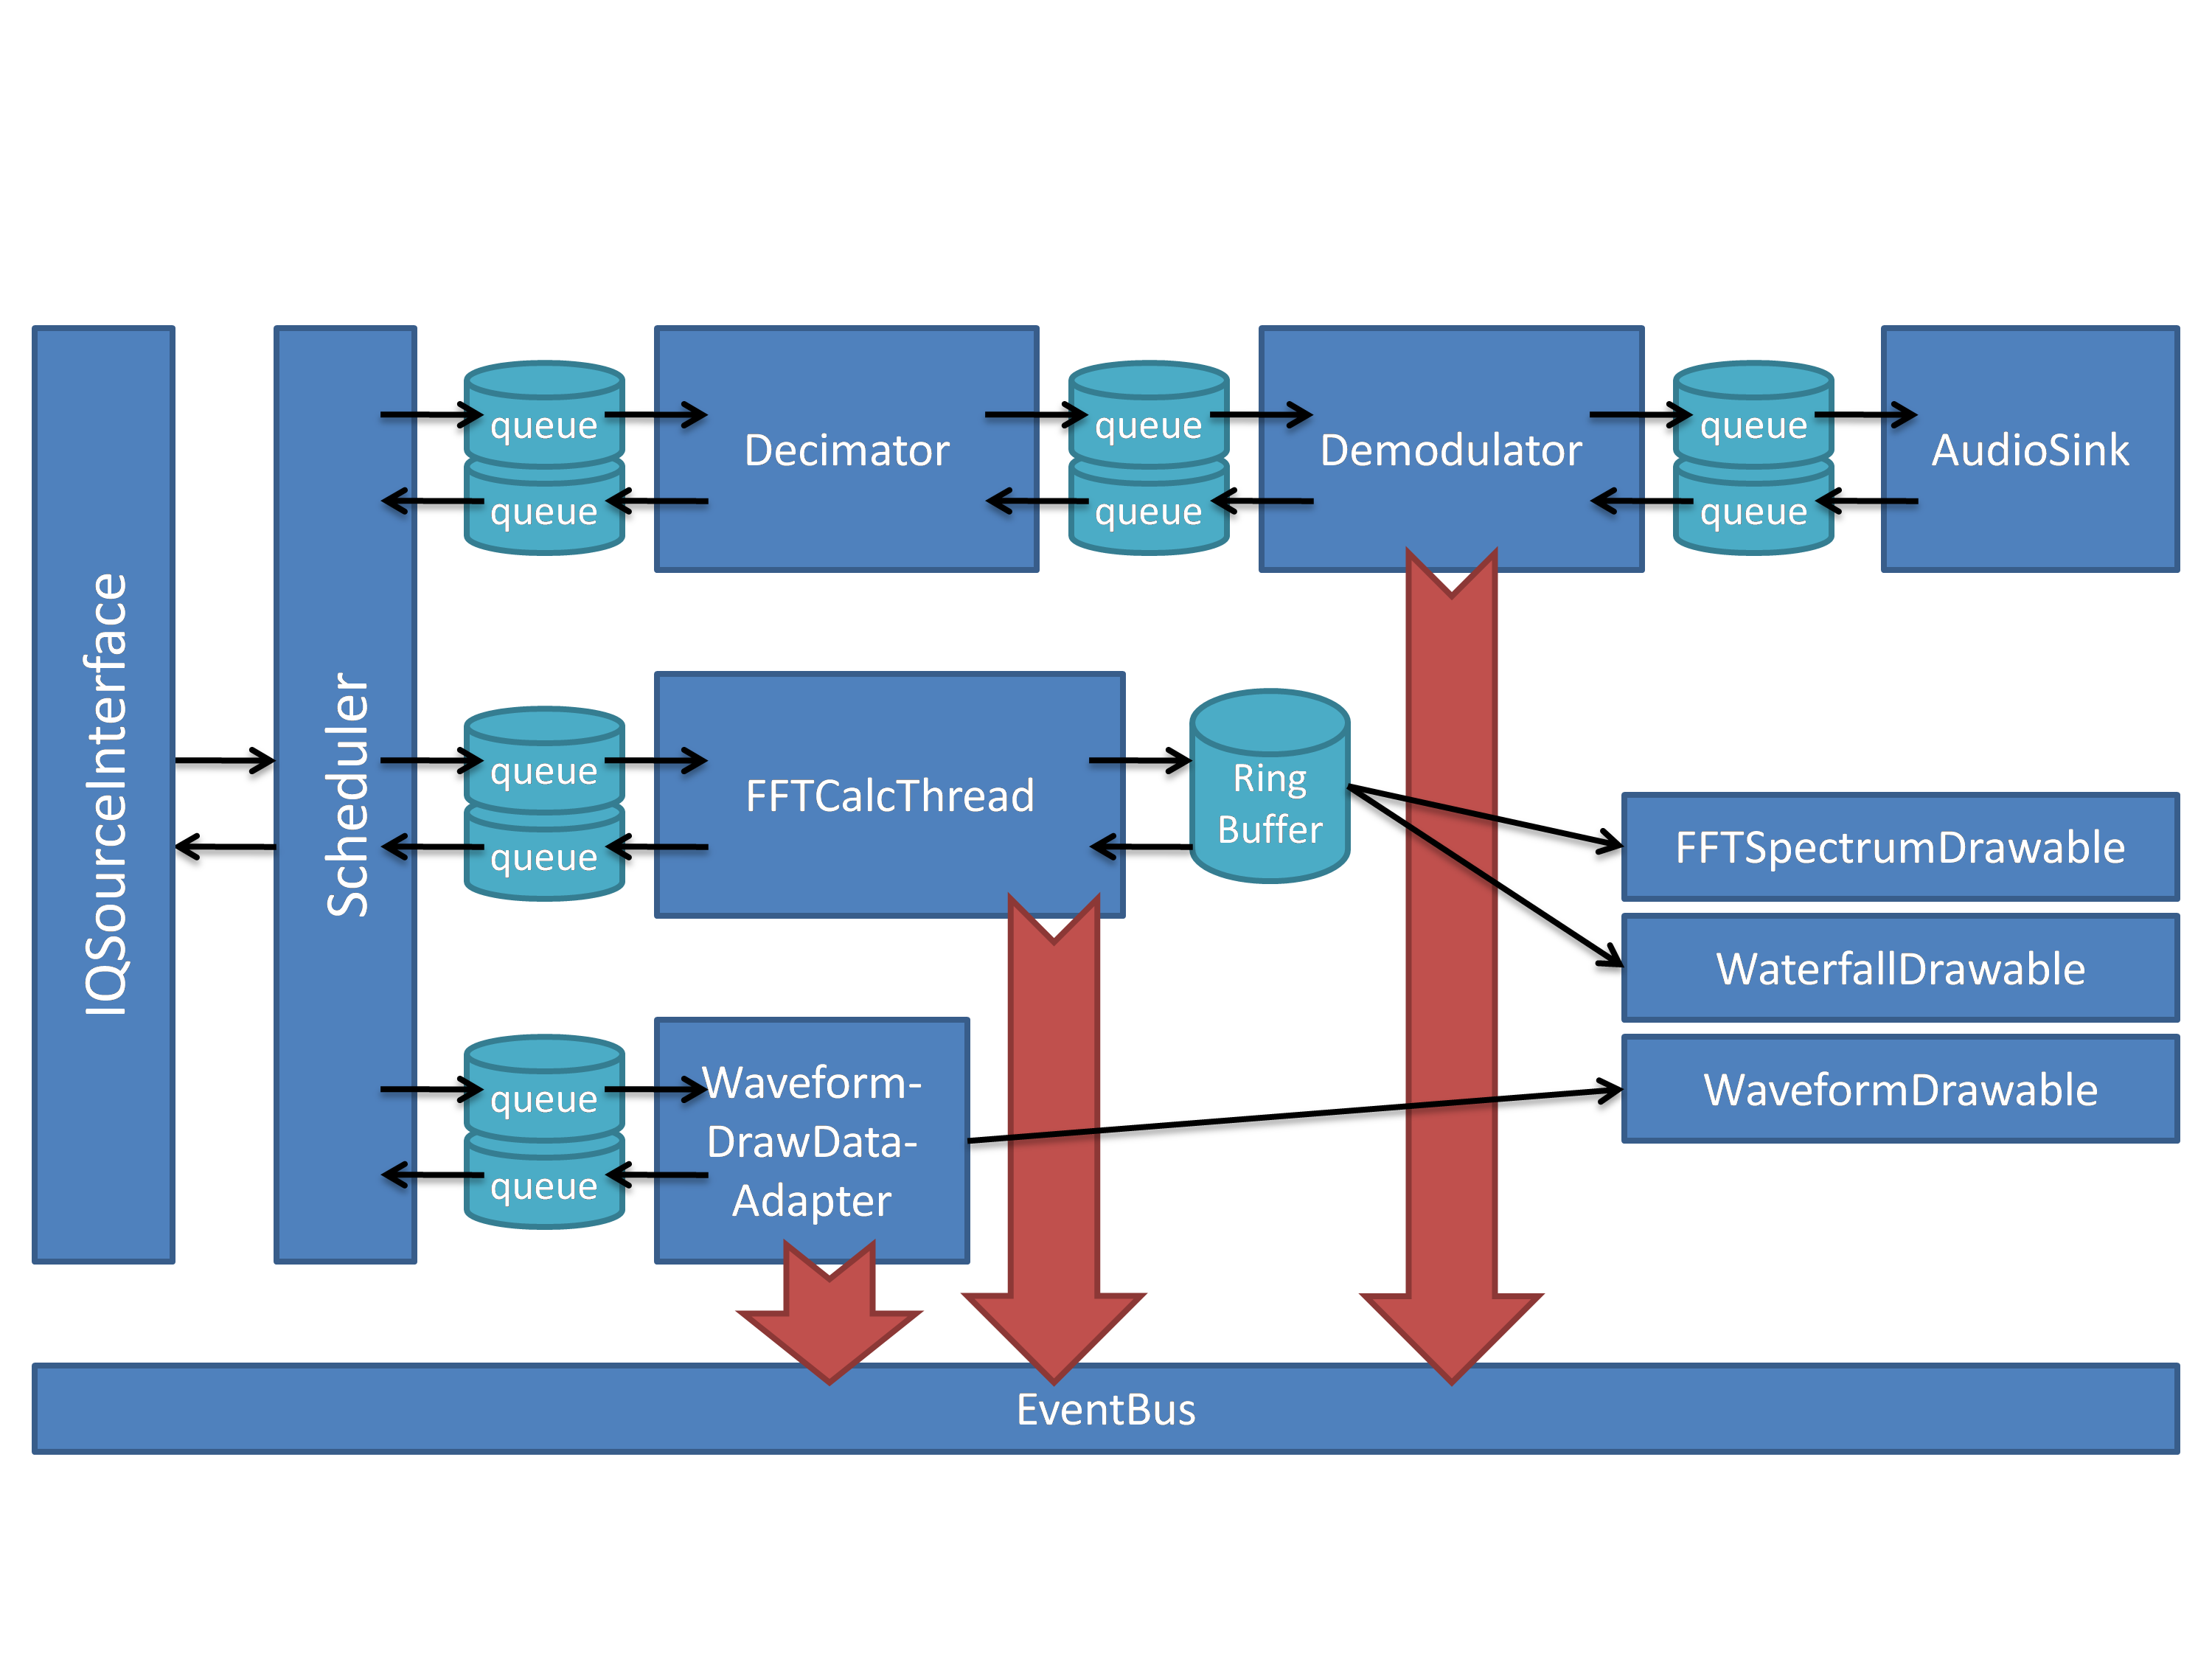
\includegraphics[width=1\linewidth]{gfx/queue_arch}
	\caption{Signal processing architecture with blocking queues}
	\label{fig:queue_architecture}
\end{figure}

The original RF Analyzer application's architecture is based on
blocking queues that synchronize the various signal processing threads
and efficiently manage memory buffers. Unfortunately, this
architecture was partly dropped by the developers of \ac{AnSiAn} when
changing to a new architecture based on the EventBus library. As a result, memory
allocation management does not work as efficiently with the current version
of \ac{AnSiAn}.

Instead of using cycling buffers for inter-thread-communication, \ac{AnSiAn} uses
EventBus to deliver data. Buffers are always allocated freshly
and discarded after use. This results in a high activity of the
\ac{GC} and therefore in a bad overall performance of the app.

\autoref{lst:before_mem_optimization} shows a logcat output of the
app before any optimizations were applied. The \ac{GC} runs approximately 8 times per second
and the slow performance results in stuttering audio demodulation on
older hardware.

\begin{lstlisting}[label=lst:before_mem_optimization, caption=Logcat output
before memory optimizations, language=none]
05-12 17:55:04.060 D/dalvikvm: GC_FOR_ALLOC freed 4347K, 14% free 54695K/62984K, paused 28ms, total 28ms
05-12 17:55:04.180 D/dalvikvm: GC_FOR_ALLOC freed 4321K, 14% free 54737K/62984K, paused 26ms, total 26ms
05-12 17:55:04.300 D/dalvikvm: GC_FOR_ALLOC freed 4507K, 14% free 54705K/62984K, paused 32ms, total 32ms
05-12 17:55:04.420 D/dalvikvm: GC_FOR_ALLOC freed 4454K, 14% free 54759K/62984K, paused 30ms, total 30ms
\end{lstlisting}

In order to fix this performance issue, the architecture is reverted
to using blocking queues and cycling buffers in places where large memory buffers are passed
between threads. EventBus is still used for delivering information
which is not tied to large buffers. A schema of the new architecture
is depicted in \autoref{fig:queue_architecture}. 

In this architecture, the buffers cycle between the threads. The re-usage
of buffers helps to reduce the memory allocation and garbage collection
overhead to a minimum. \autoref{lst:after_mem_optimization} shows the
logcat output after the architecture changes have been applied. The \ac{GC}
only needs to run every 10 to 20 seconds.


\begin{lstlisting}[label=lst:after_mem_optimization, caption=Logcat output
after memory optimizations, language=none]
05-12 17:27:29.230 D/dalvikvm: GC_FOR_ALLOC freed 3233K, 15% free 19706K/23000K, paused 32ms, total 33ms
05-12 17:27:40.780 D/dalvikvm: GC_FOR_ALLOC freed 3528K, 16% free 20235K/23824K, paused 30ms, total 31ms
05-12 17:28:00.110 D/dalvikvm: GC_FOR_ALLOC freed 4130K, 18% free 20338K/24528K, paused 36ms, total 37ms
05-12 17:28:24.520 D/dalvikvm: GC_FOR_ALLOC freed 4263K, 18% free 20341K/24664K, paused 49ms, total 49ms
\end{lstlisting}


%%*****************************************
%\chapter{Related Work}\label{ch:relatedwork}
%%*****************************************
%\glsresetall % Resets all acronyms to not used
%
%\lipsum[4]
